\documentclass{article}\usepackage[]{graphicx}\usepackage[]{color}
% maxwidth is the original width if it is less than linewidth
% otherwise use linewidth (to make sure the graphics do not exceed the margin)
\makeatletter
\def\maxwidth{ %
  \ifdim\Gin@nat@width>\linewidth
    \linewidth
  \else
    \Gin@nat@width
  \fi
}
\makeatother

\definecolor{fgcolor}{rgb}{0.345, 0.345, 0.345}
\newcommand{\hlnum}[1]{\textcolor[rgb]{0.686,0.059,0.569}{#1}}%
\newcommand{\hlstr}[1]{\textcolor[rgb]{0.192,0.494,0.8}{#1}}%
\newcommand{\hlcom}[1]{\textcolor[rgb]{0.678,0.584,0.686}{\textit{#1}}}%
\newcommand{\hlopt}[1]{\textcolor[rgb]{0,0,0}{#1}}%
\newcommand{\hlstd}[1]{\textcolor[rgb]{0.345,0.345,0.345}{#1}}%
\newcommand{\hlkwa}[1]{\textcolor[rgb]{0.161,0.373,0.58}{\textbf{#1}}}%
\newcommand{\hlkwb}[1]{\textcolor[rgb]{0.69,0.353,0.396}{#1}}%
\newcommand{\hlkwc}[1]{\textcolor[rgb]{0.333,0.667,0.333}{#1}}%
\newcommand{\hlkwd}[1]{\textcolor[rgb]{0.737,0.353,0.396}{\textbf{#1}}}%
\let\hlipl\hlkwb

\usepackage{framed}
\makeatletter
\newenvironment{kframe}{%
 \def\at@end@of@kframe{}%
 \ifinner\ifhmode%
  \def\at@end@of@kframe{\end{minipage}}%
  \begin{minipage}{\columnwidth}%
 \fi\fi%
 \def\FrameCommand##1{\hskip\@totalleftmargin \hskip-\fboxsep
 \colorbox{shadecolor}{##1}\hskip-\fboxsep
     % There is no \\@totalrightmargin, so:
     \hskip-\linewidth \hskip-\@totalleftmargin \hskip\columnwidth}%
 \MakeFramed {\advance\hsize-\width
   \@totalleftmargin\z@ \linewidth\hsize
   \@setminipage}}%
 {\par\unskip\endMakeFramed%
 \at@end@of@kframe}
\makeatother

\definecolor{shadecolor}{rgb}{.97, .97, .97}
\definecolor{messagecolor}{rgb}{0, 0, 0}
\definecolor{warningcolor}{rgb}{1, 0, 1}
\definecolor{errorcolor}{rgb}{1, 0, 0}
\newenvironment{knitrout}{}{} % an empty environment to be redefined in TeX

\usepackage{alltt}
\usepackage{graphicx}
%% for inline R code: if the inline code is not correctly parsed, you will see a message
\newcommand{\rinline}[1]{SOMETHING WRONG WITH knitr}


\IfFileExists{upquote.sty}{\usepackage{upquote}}{}
\begin{document}

Boring stuff as usual:

%% a chunk with default options
\begin{knitrout}
\definecolor{shadecolor}{rgb}{0.969, 0.969, 0.969}\color{fgcolor}\begin{kframe}
\begin{alltt}
 \hlnum{1}\hlopt{+}\hlnum{1}
\end{alltt}
\begin{verbatim}
## [1] 2
\end{verbatim}
\begin{alltt}
 \hlstd{x}\hlkwb{=}\hlkwd{rnorm}\hlstd{(}\hlnum{5}\hlstd{)}
\end{alltt}
\end{kframe}
\end{knitrout}

For the cached chunk below, you will need to wait for 10 seconds for
the first time you compile this document, but it takes no time the
next time you run it again.

%% chunk options: cache this chunk
\begin{knitrout}
\definecolor{shadecolor}{rgb}{0.969, 0.969, 0.969}\color{fgcolor}\begin{kframe}
\begin{alltt}
 \hlkwd{set.seed}\hlstd{(}\hlnum{123}\hlstd{)}
 \hlstd{x} \hlkwb{=} \hlkwd{runif}\hlstd{(}\hlnum{10}\hlstd{)}
 \hlkwd{sd}\hlstd{(x)}  \hlcom{# standard deviation}
\end{alltt}
\begin{verbatim}
## [1] 0.29474
\end{verbatim}
\begin{alltt}
 \hlkwd{Sys.sleep}\hlstd{(}\hlnum{10}\hlstd{)} \hlcom{# test cache}
\end{alltt}
\end{kframe}
\end{knitrout}

Now we know the first element of x is 0.2875775. And we also know
the 26 letters are A, B, C, D, E, F, G, H, I, J, K, L, M, N, O, P, Q, R, S, T, U, V, W, X, Y, Z. An expression that returns a
value of length 0 will be removed from the output,  but it was indeed evaluated, e.g. now the first element
of x becomes 2011.

How about figures? Let's use the Cairo PDF device (assumes R $\geq$
2.14.0).

\begin{knitrout}
\definecolor{shadecolor}{rgb}{0.969, 0.969, 0.969}\color{fgcolor}\begin{kframe}
\begin{alltt}
\hlkwd{plot}\hlstd{(cars)} \hlcom{# a scatter plot}
\end{alltt}
\end{kframe}
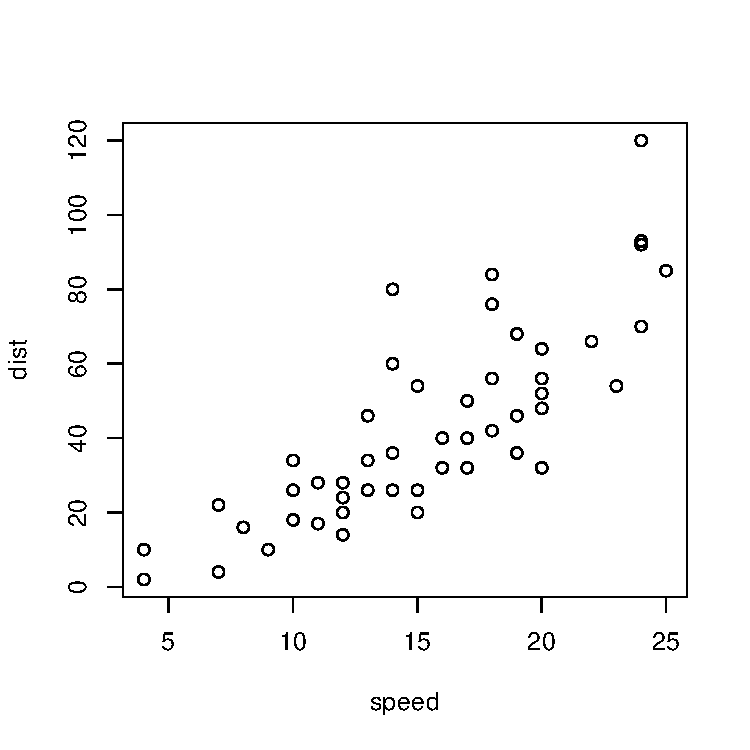
\includegraphics[width=.8\textwidth]{figure/latex-cairo-scatter-1} 

\end{knitrout}

Warnings, messages and errors are preserved by default.

\begin{knitrout}
\definecolor{shadecolor}{rgb}{0.969, 0.969, 0.969}\color{fgcolor}\begin{kframe}
\begin{alltt}
\hlkwd{sqrt}\hlstd{(}\hlopt{-}\hlnum{1}\hlstd{)} \hlcom{# here is a warning!}
\end{alltt}


{\ttfamily\noindent\color{warningcolor}{\#\# Warning in sqrt(-1): NaNs produced}}\begin{verbatim}
## [1] NaN
\end{verbatim}
\begin{alltt}
\hlkwd{message}\hlstd{(}\hlstr{'this is a message you should know'}\hlstd{)}
\end{alltt}


{\ttfamily\noindent\itshape\color{messagecolor}{\#\# this is a message you should know}}\begin{alltt}
\hlnum{1}\hlopt{+}\hlstr{'a'}  \hlcom{# impossible}
\end{alltt}


{\ttfamily\noindent\bfseries\color{errorcolor}{\#\# Error in 1 + "{}a"{}: non-numeric argument to binary operator}}\end{kframe}
\end{knitrout}

\end{document}
